\documentclass[titlepage, 12pt]{article}

\usepackage{framed}
\usepackage{enumitem}
\usepackage{geometry}
\geometry{
  letterpaper,
  margin=1in,
}

\usepackage{graphicx}
\graphicspath{{./images/}}
\usepackage{float}

\title{SE 2XB3 Group 4 Report 2}
\author{
  Huang, Kehao \\
  400235182 \\
  \texttt{huangk53@mcmaster.ca} \\
  L01
  \and
  Jiao, Anhao \\
  400251837 \\
  \texttt{jiaoa3@mcmaster.ca} \\
  L01
  \and
  Ye, Xunzhou \\
  400268576 \\
  \texttt{yex33@mcmaster.ca} \\
  L01
}
\date{\today}

\begin{document}
\maketitle{}

\newpage{}

\section{Timeing Data}

\subsection{$f(n)$ Analysis}

$f(n)$ is determined to be growing in the order of $\mathcal{O}(n)$. We started
by plotting $f(n)$ on a x-y plane and observed a graph similar to that of a
linear function. We formed our speculation on $f(n)$ being linear. A linear
regression on the data set was then attempted to further investigate. As shown
in Figure \ref{fig:fn-linreg}, the coefficient of determination is 0.9992,
indicating that there is a high chance that $f(n)$ is indeed a linear function.
To confirm our guesses, we plotted a log-log graph for $f(n)$ in Figure
\ref{fig:fn-log-linreg}, and performed linear regression on the plot. Both the
slope of the trend line and the $R^{2}$ value were approximately 0.9994. This is
strong evidence that $f(n)$ grows in the order of $\mathcal{O}(n)$.
\begin{figure}[H]
    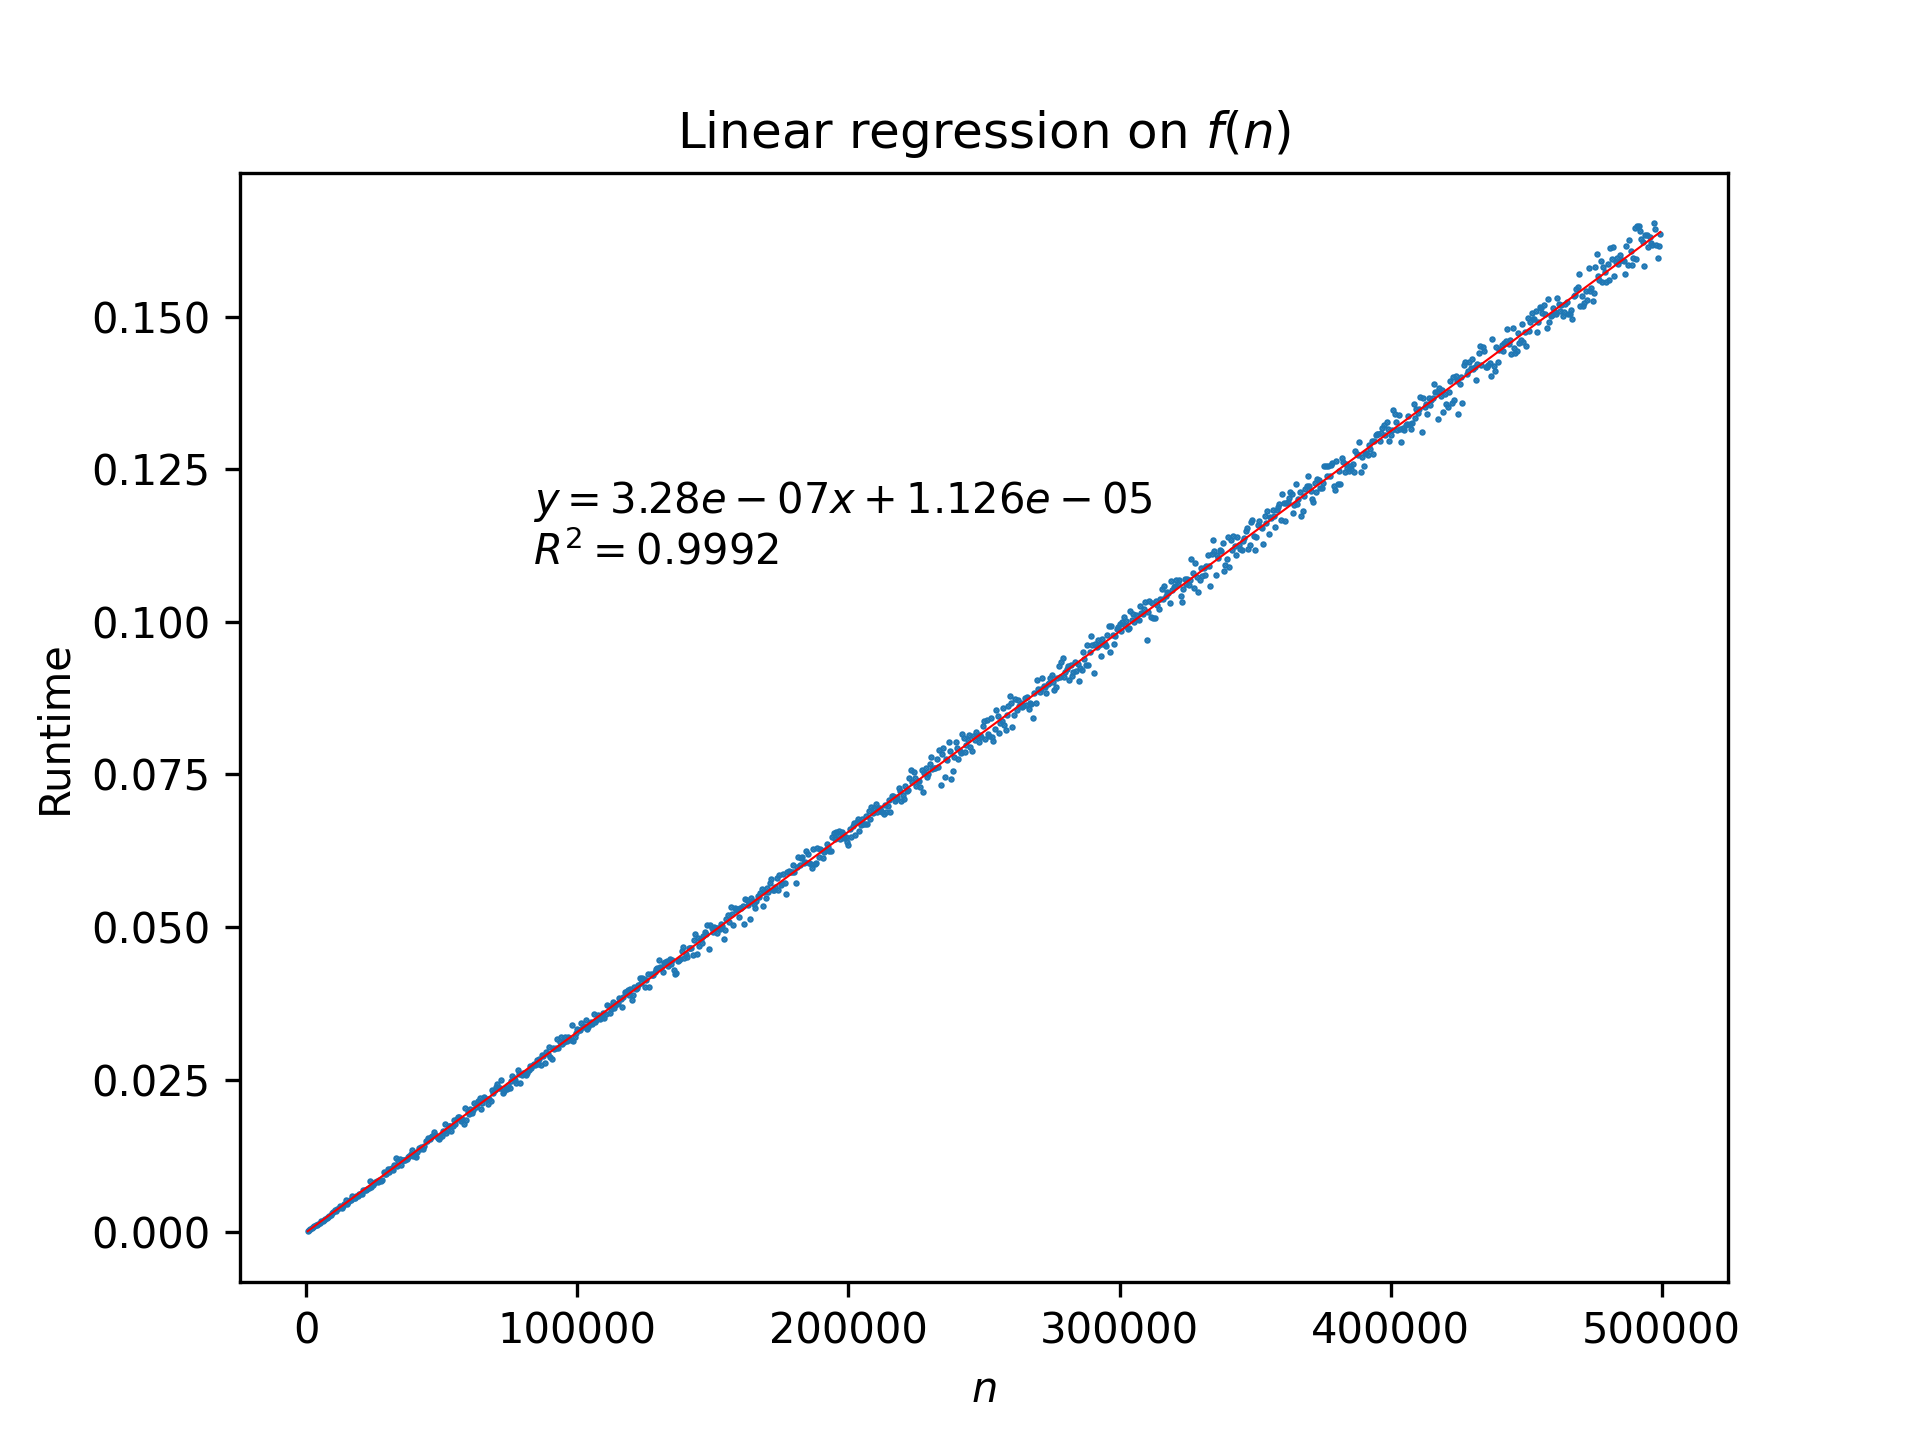
\includegraphics[width=0.8\linewidth]{fn-linreg.png}
    \centering
    \caption{$f(n)$ linear regression}
    \label{fig:fn-linreg} 
\end{figure}
\begin{figure}[H]
    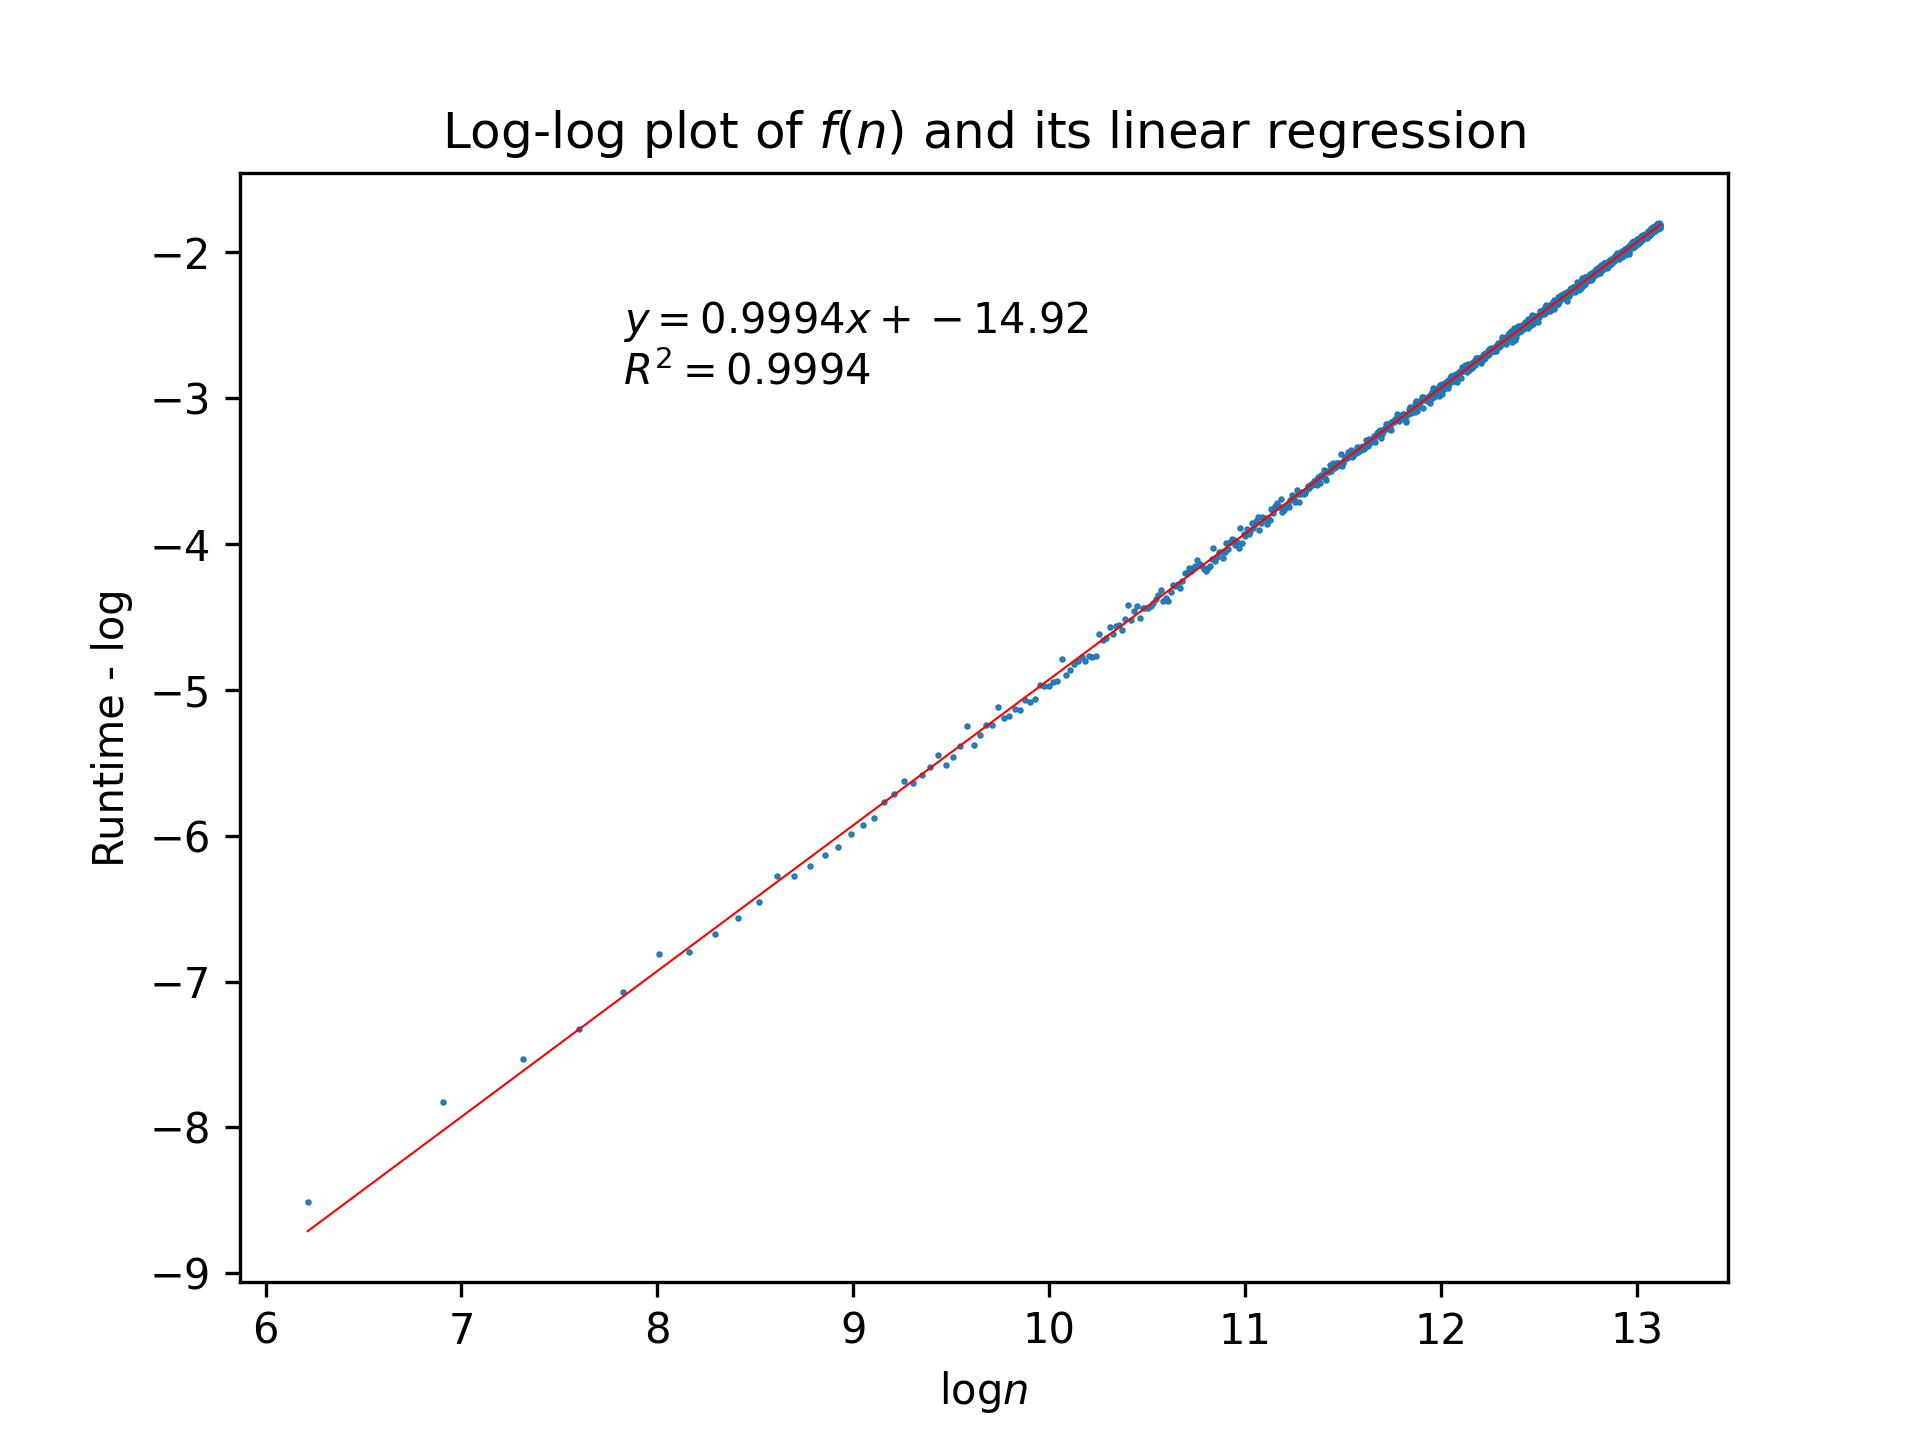
\includegraphics[width=0.8\linewidth]{fn-log-linreg.png}
    \centering
    \caption{$f(n)$ log-log plot}
    \label{fig:fn-log-linreg}
\end{figure}

\subsection{$g(n)$ Analysis}
By observing the graph of $g(n)$, our guess on the order of growth was
polynomial or power. After applying the fitting line and constructed $R^{2}$
value, we found that the polynomial function with power of 3 fit the dots the
most. However, the coefficient of $x^{3}$ is relatively smaller than the
coefficient of $x^{2}$. To confirm our hypothesis on the growth order, we
plotted the log graph and resulted in a linear regression with 2.8548 as the
coefficient of $x$. Because there were nly 43 pairs of data were given for
$g(n)$, so the insufficient amount of data ould cause the difference between
2.8548 and 3(the expected growth rate). Overall, with the finite given date set,
we concluded that $g(n)$ has a growth order of $\mathcal{O}(x^{3})$
\begin{figure}[H]
    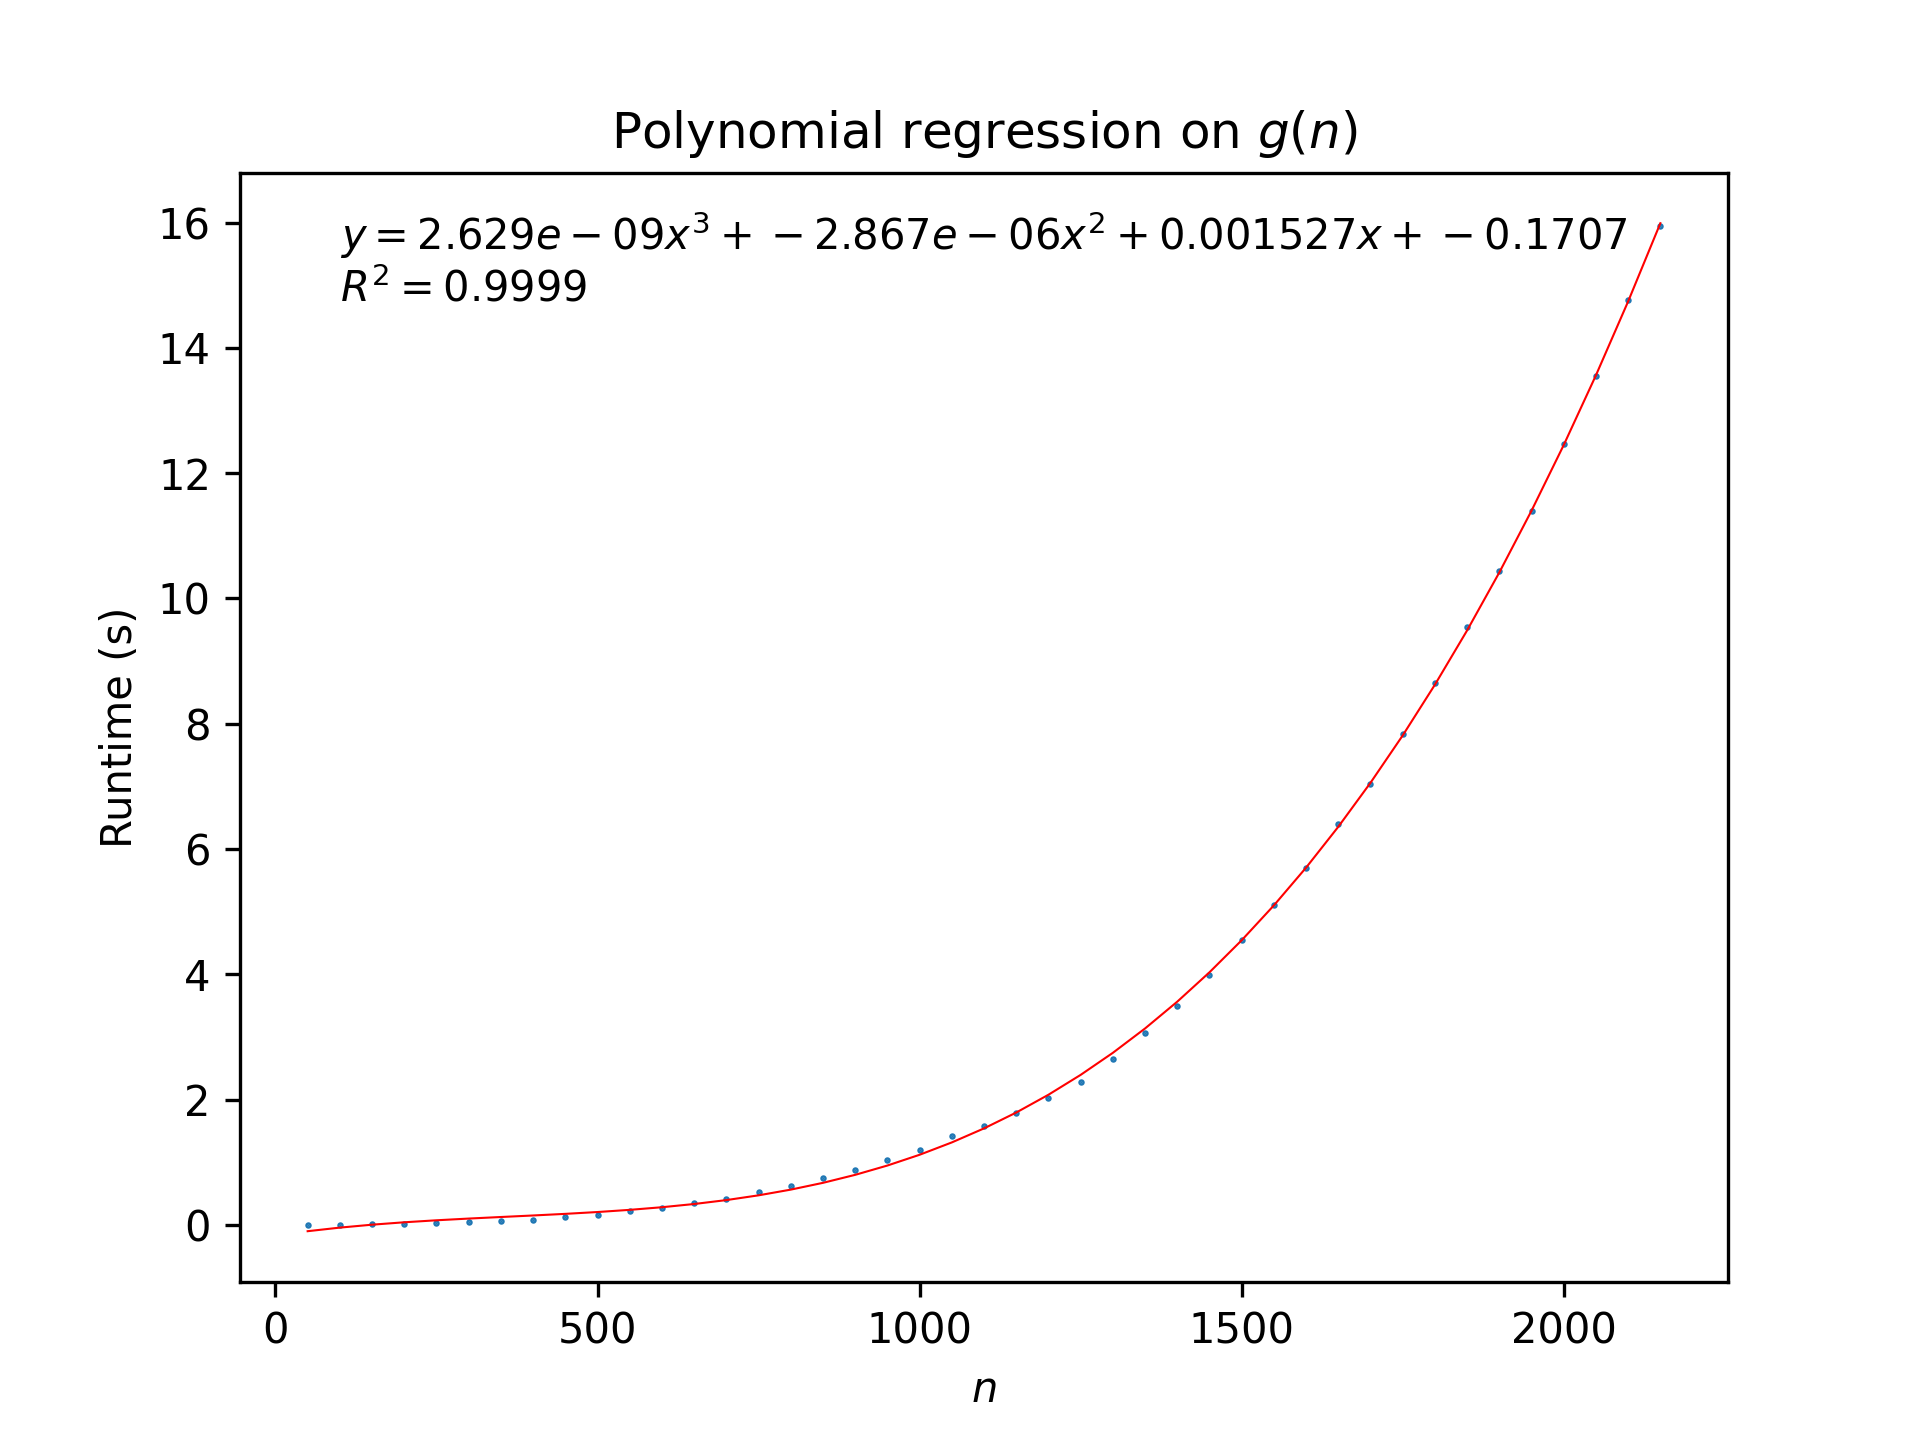
\includegraphics[width=0.8\linewidth]{gn-polyreg.png}
    \centering
    \caption{$g(n)$ polynomial regression}
    \label{fig:gn-polyreg}
\end{figure}
\begin{figure}[H]
    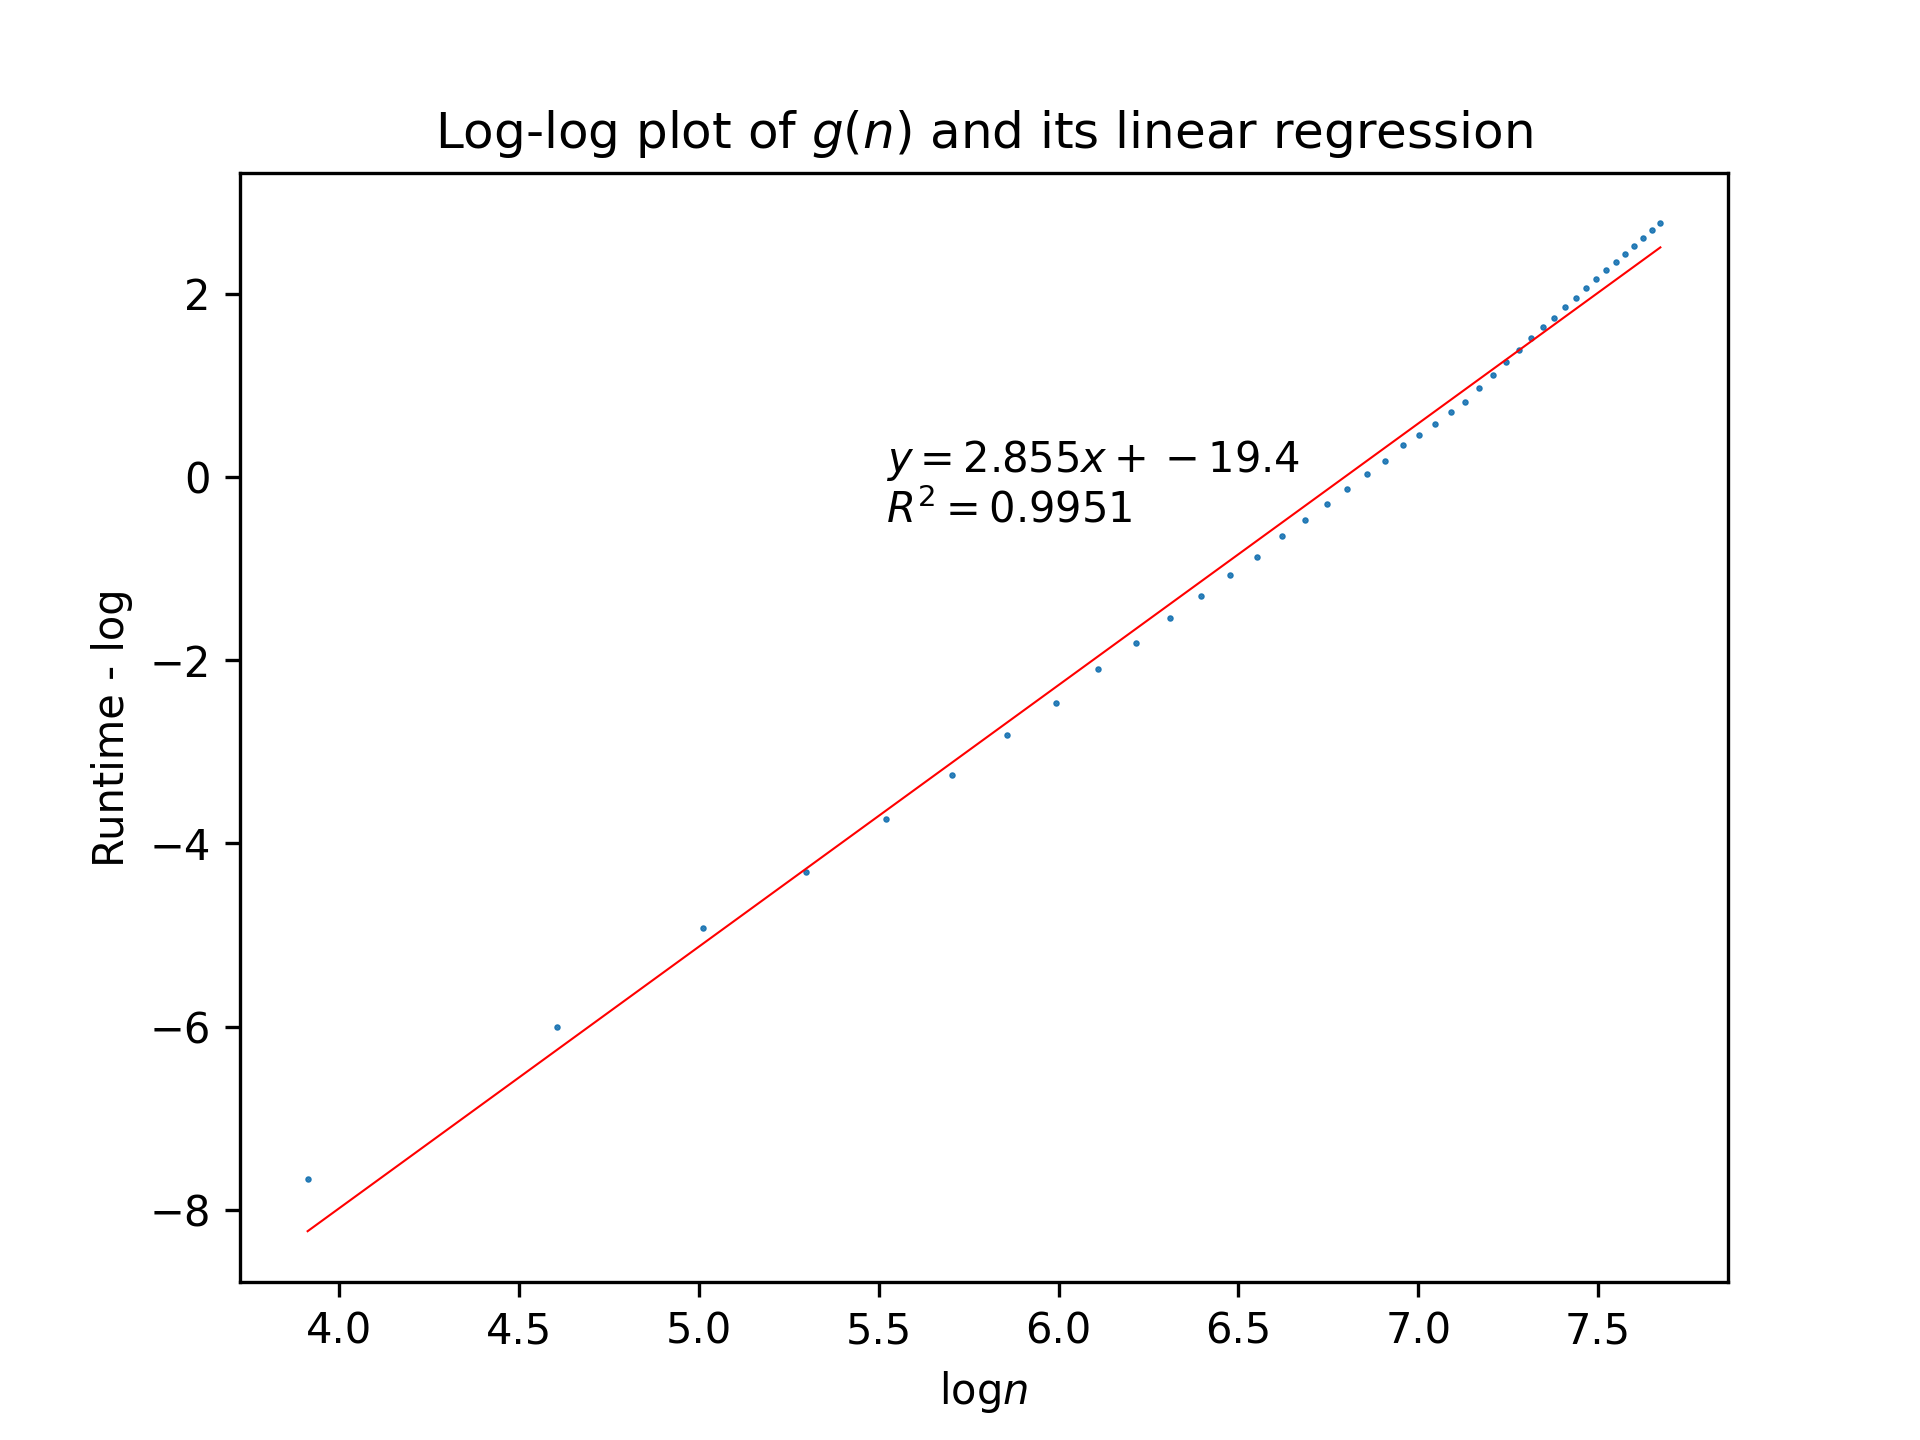
\includegraphics[width=0.8\linewidth]{gn-log-linreg.png}
    \centering
    \caption{$g(n)$ log-log plot}
    \label{fig:gn-log-linreg}
\end{figure}

\subsection{$h(n)$ Analysis}
After plotting the $h(n)$ data set into the graph, our first intuition about the
type of growth was linear. However, by the visual contrast with the $h(n)$ in
Figure \ref{fig:hn-polyreg}, we all thought that the fitting line bended too
much as a linear function. Therefore, we made the second graph which plotted
with $log(n)$ and $log(runtime)$ in Figure \ref{fig:hn-log-linreg}, as the
x-axis and the y-axis respectively. Then, we analyzed the coefficient of the
term that has the highest power($x$). Compared to 1, the coefficient 1.1069 is
off by quite a bit. At this point we were uncertain about the intuition we had
at the beginning. Because the coefficient is larger than 1 which means it grows
faster than linear, however, not as much as polynomial, exponential or power
functions. At this point, we doubted that it could be $nlog(n)$ form. Last but
not least, we divided the runtime($nlog(n)$) by its number($n$) and we got a
$logn$ graph in Figure \ref{fig:hn-over-n-logreg}. Our assumption was right and
the graph fits as a log function. In conclusion, the $h(n)$ grows in the order
of $\mathcal{O}(nlog(n))$
\begin{figure}[H]
  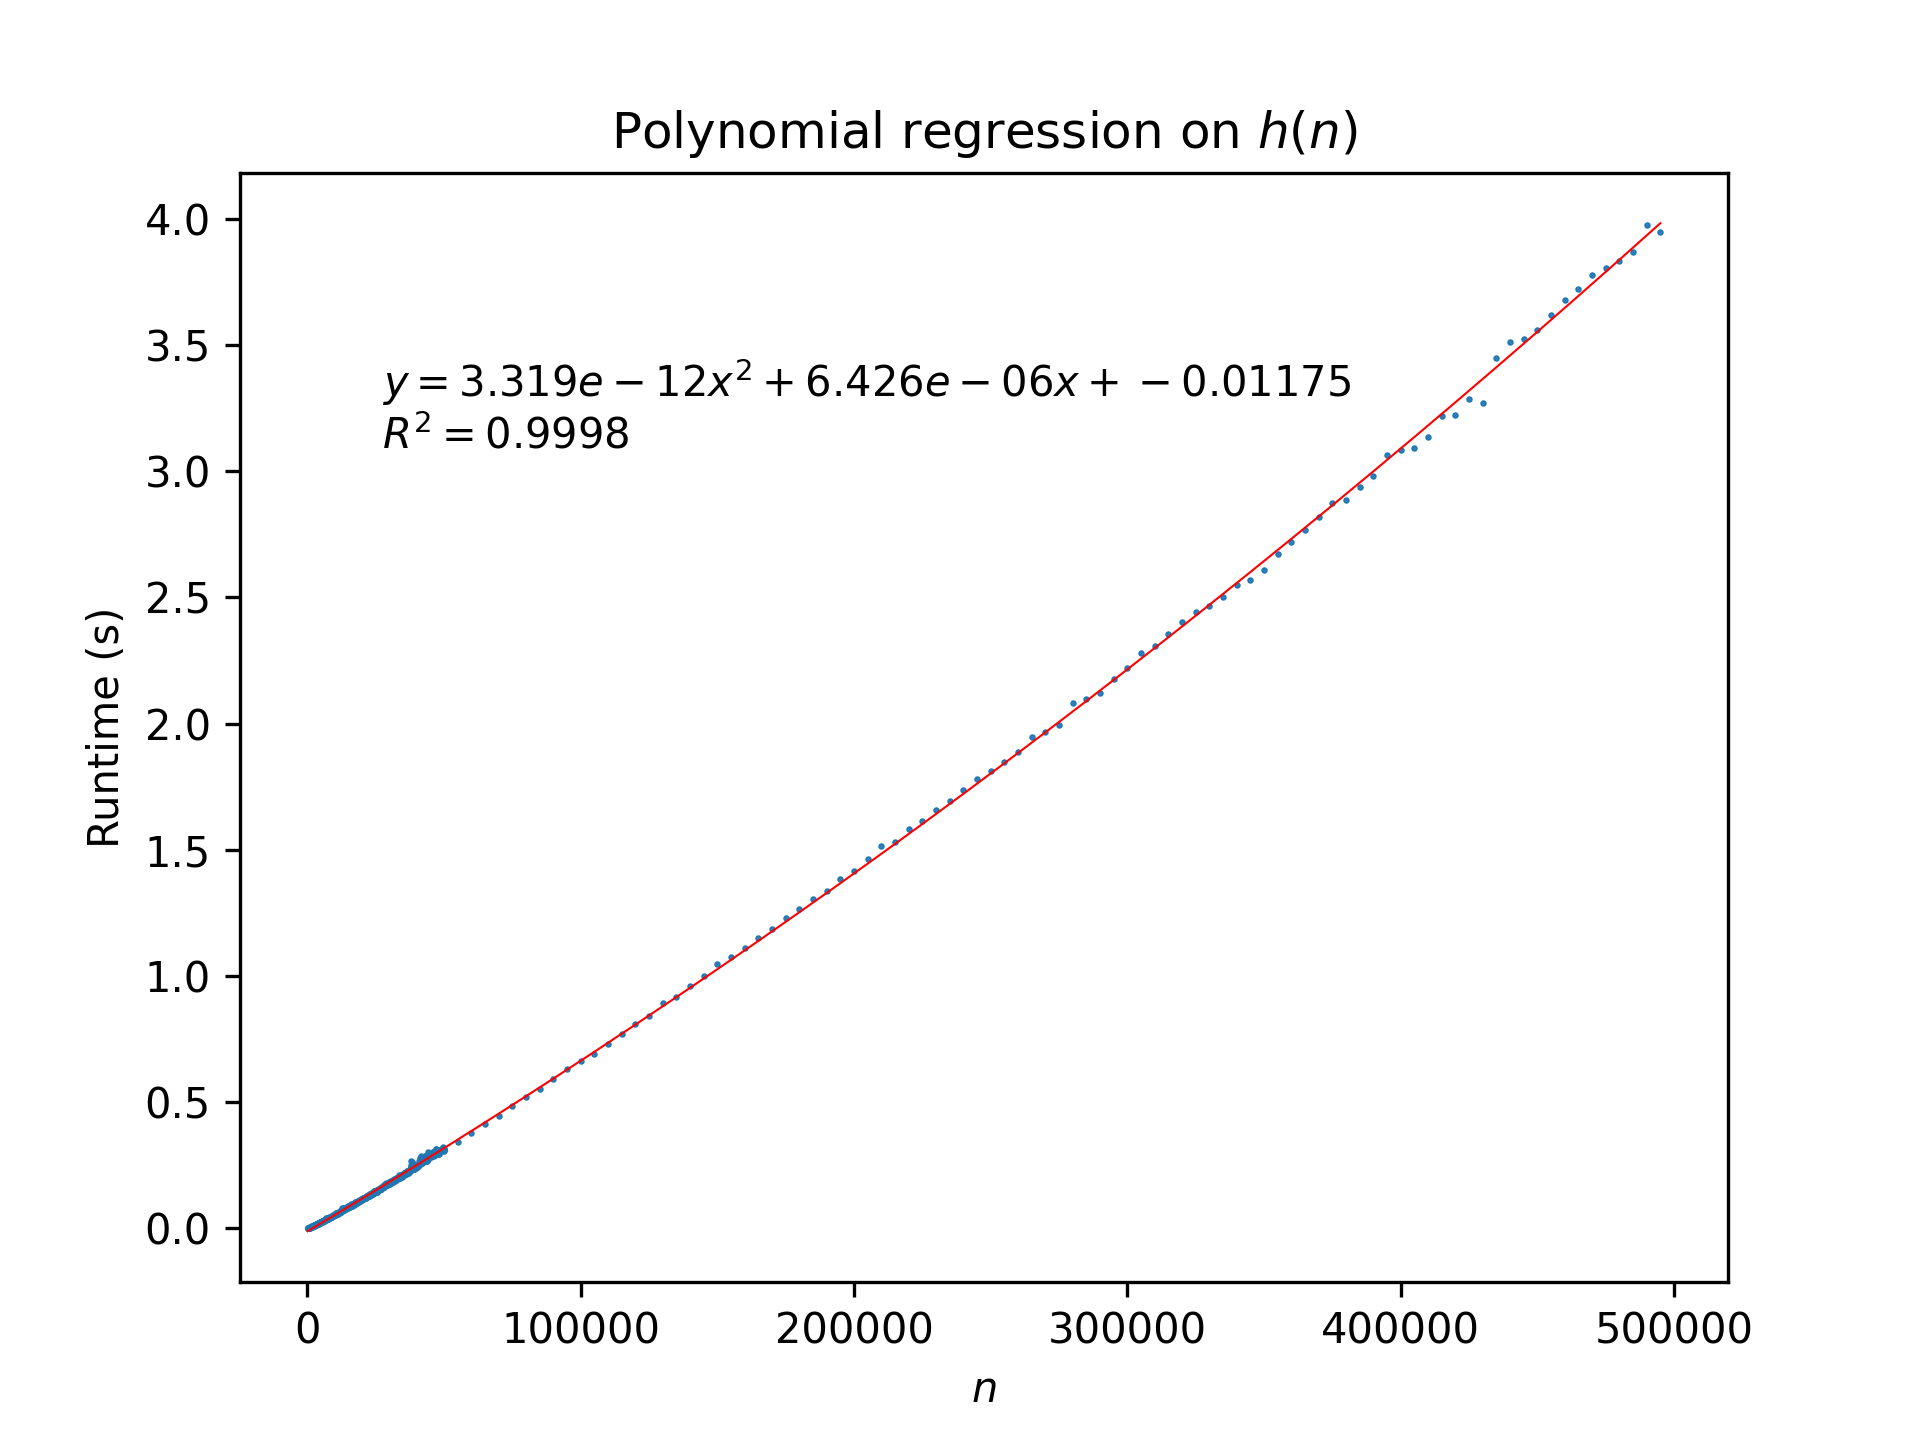
\includegraphics[width=0.8\linewidth]{hn-polyreg.png}
  \centering
  \caption{$h(n)$ polynomial regression}
  \label{fig:hn-polyreg}
\end{figure}
\begin{figure}[H]
  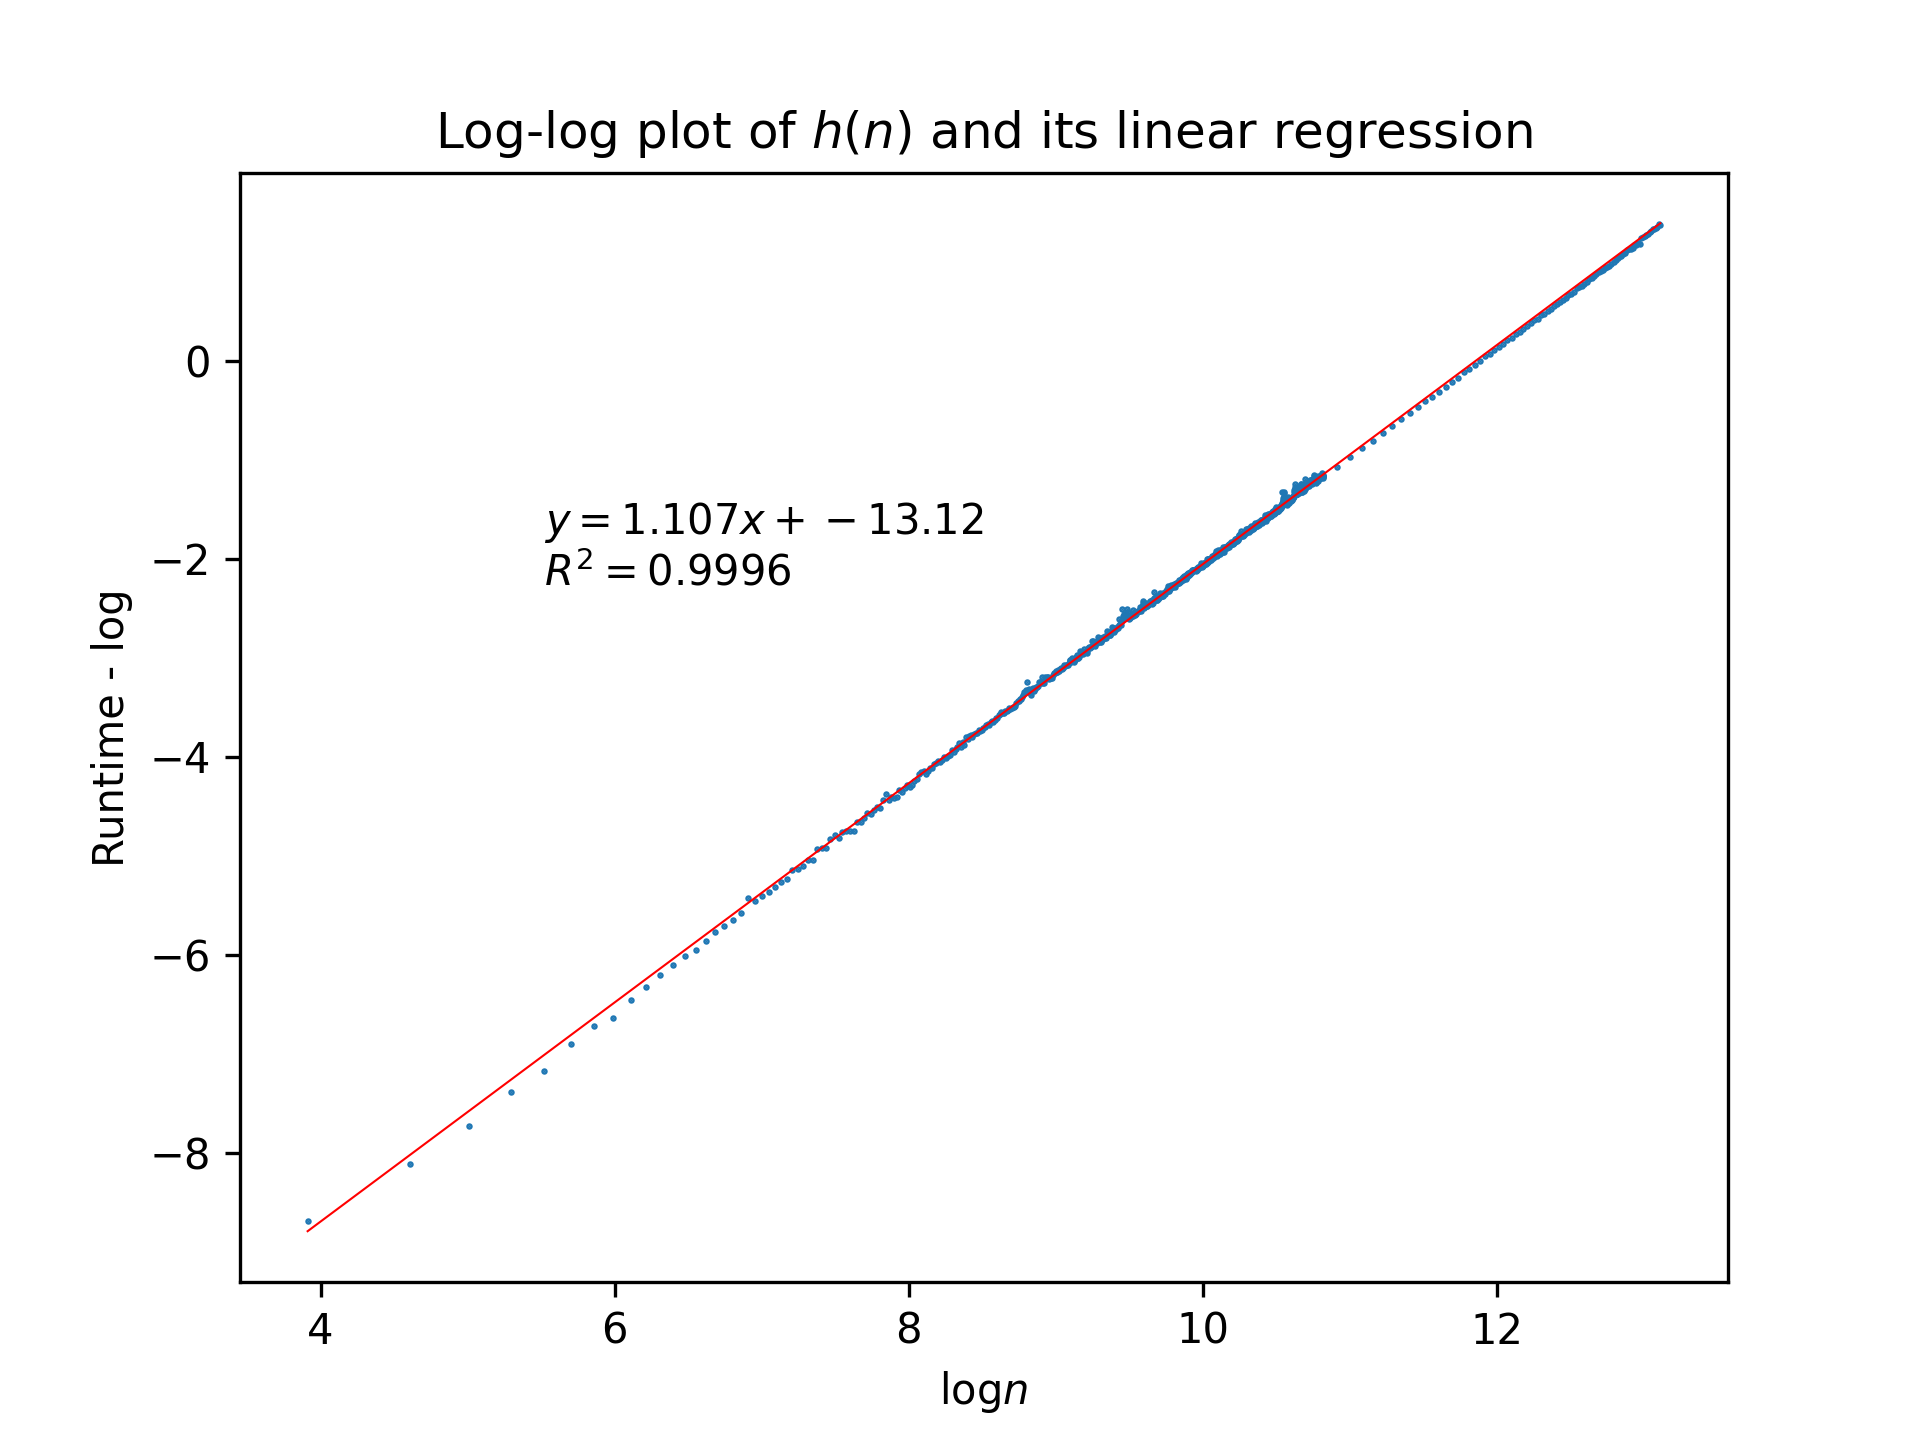
\includegraphics[width=0.8\linewidth]{hn-log-linreg.png}
  \centering
  \caption{$h(n)$ log-log plot}
  \label{fig:hn-log-linreg}
\end{figure}
\begin{figure}[H]
  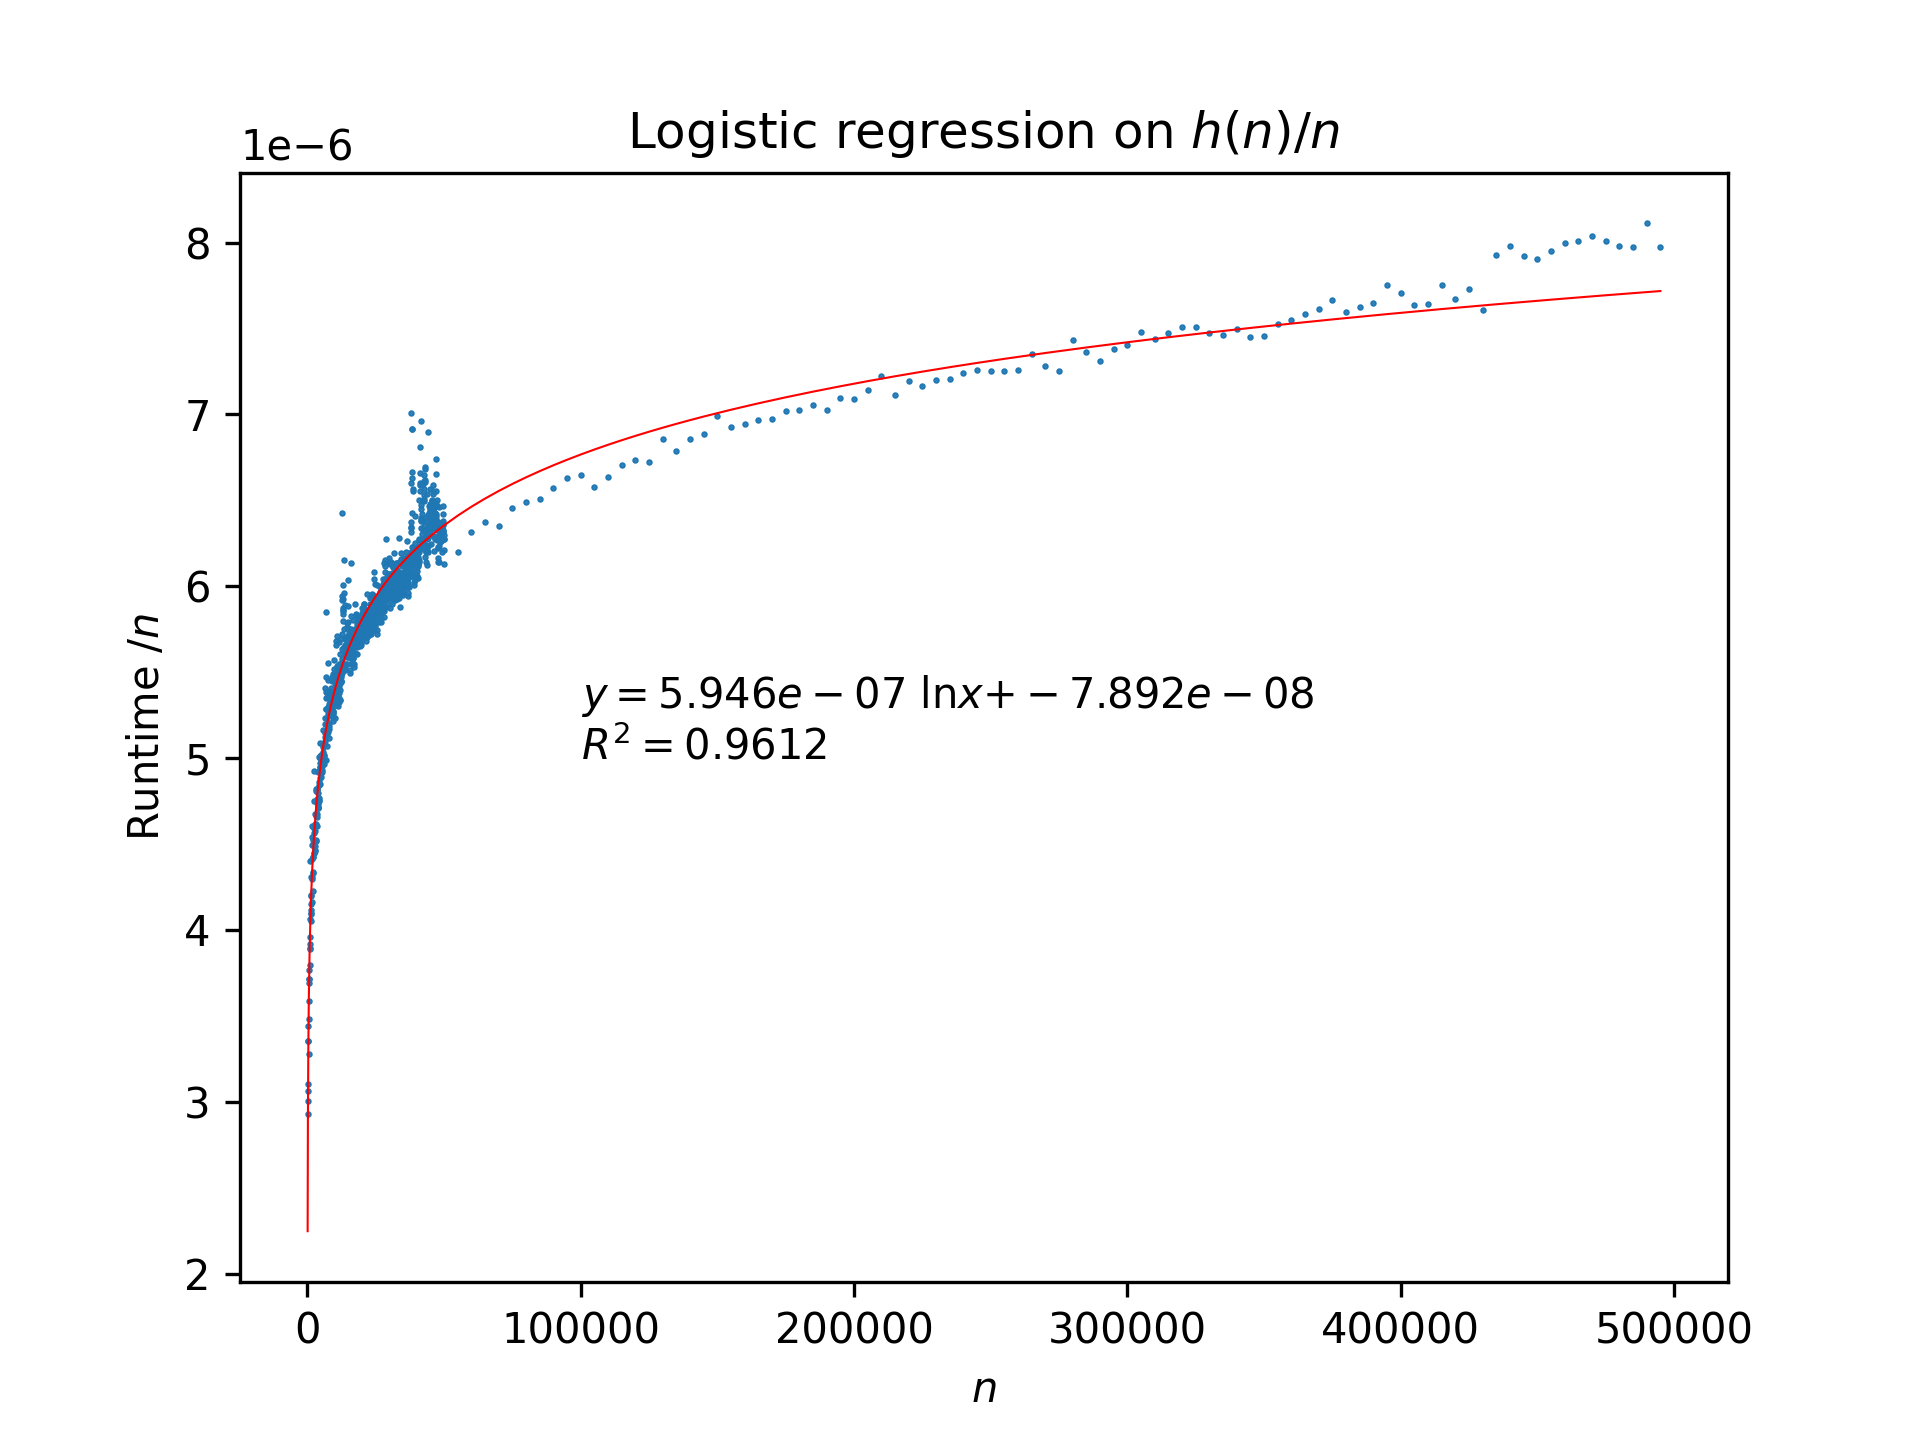
\includegraphics[width=0.8\linewidth]{hn-over-n-logreg.png}
  \centering
  \caption{$h(n)/n$ logarithmic regression}
  \label{fig:hn-over-n-logreg}
\end{figure}

\section{Python Lists}

\subsection{\texttt{list.copy}}

\subsubsection{Methodology}

We tested list.copy on lists of different lengths, ranging from 100 to 10000
with a step size of 100. For each round of the test, list.copy is called 100
times. The runtime of a round is the time required to copy one specific array
100 times. The reason for analyzing 100 list.copy calls, or in a sense
normalizing each test, instead of making a single list.copy call is because a
longer runtime helps to avoid floating point arithmetic errors from processing
extremely small float numbers. For each given list length, n, 5 rounds of tests
are carried out, and the minimum runtime out of the 5 is assigned as the runtime
of the given length. Each round of test is performed with a fresh list of n
random numbers. Inspired by the documentation for the timeit library,
calculating mean and standard deviation from multiple rounds of tests is not
very useful. In a typical case, the lowest value gives a lower bound for how
fast a machine can run a test; longer runtimes are typically not caused by
variability in Python’s speed, but by other processes interfering with the
timing accuracy. So the minimum runtime out of the 5 rounds is sufficient to
represent the other runtimes.

\subsubsection{Observations}

The regression line of the plotted dots grows in the order of \( \mathcal{O}(n)
\). The \( R^2 \) value is 0.9911\footnote{The exact value may not be matching
  with the one on the figure because the figure is generated using a new set of
  data in each run of the script.} which is close enough to 1, as shown in
Figure \ref{fig:copy-linreg}. In order to back up our expectations, we created a
log-log plot for the x and y values, in Figure . The resulting regression line
has a slope close to 1, suggesting a linear relationship between the input size
\( n \) and the function runtime. We therefore conclude that \texttt{list.copy}
grows in the order of \( \mathcal{O}(n) \)
\begin{figure}[H]
  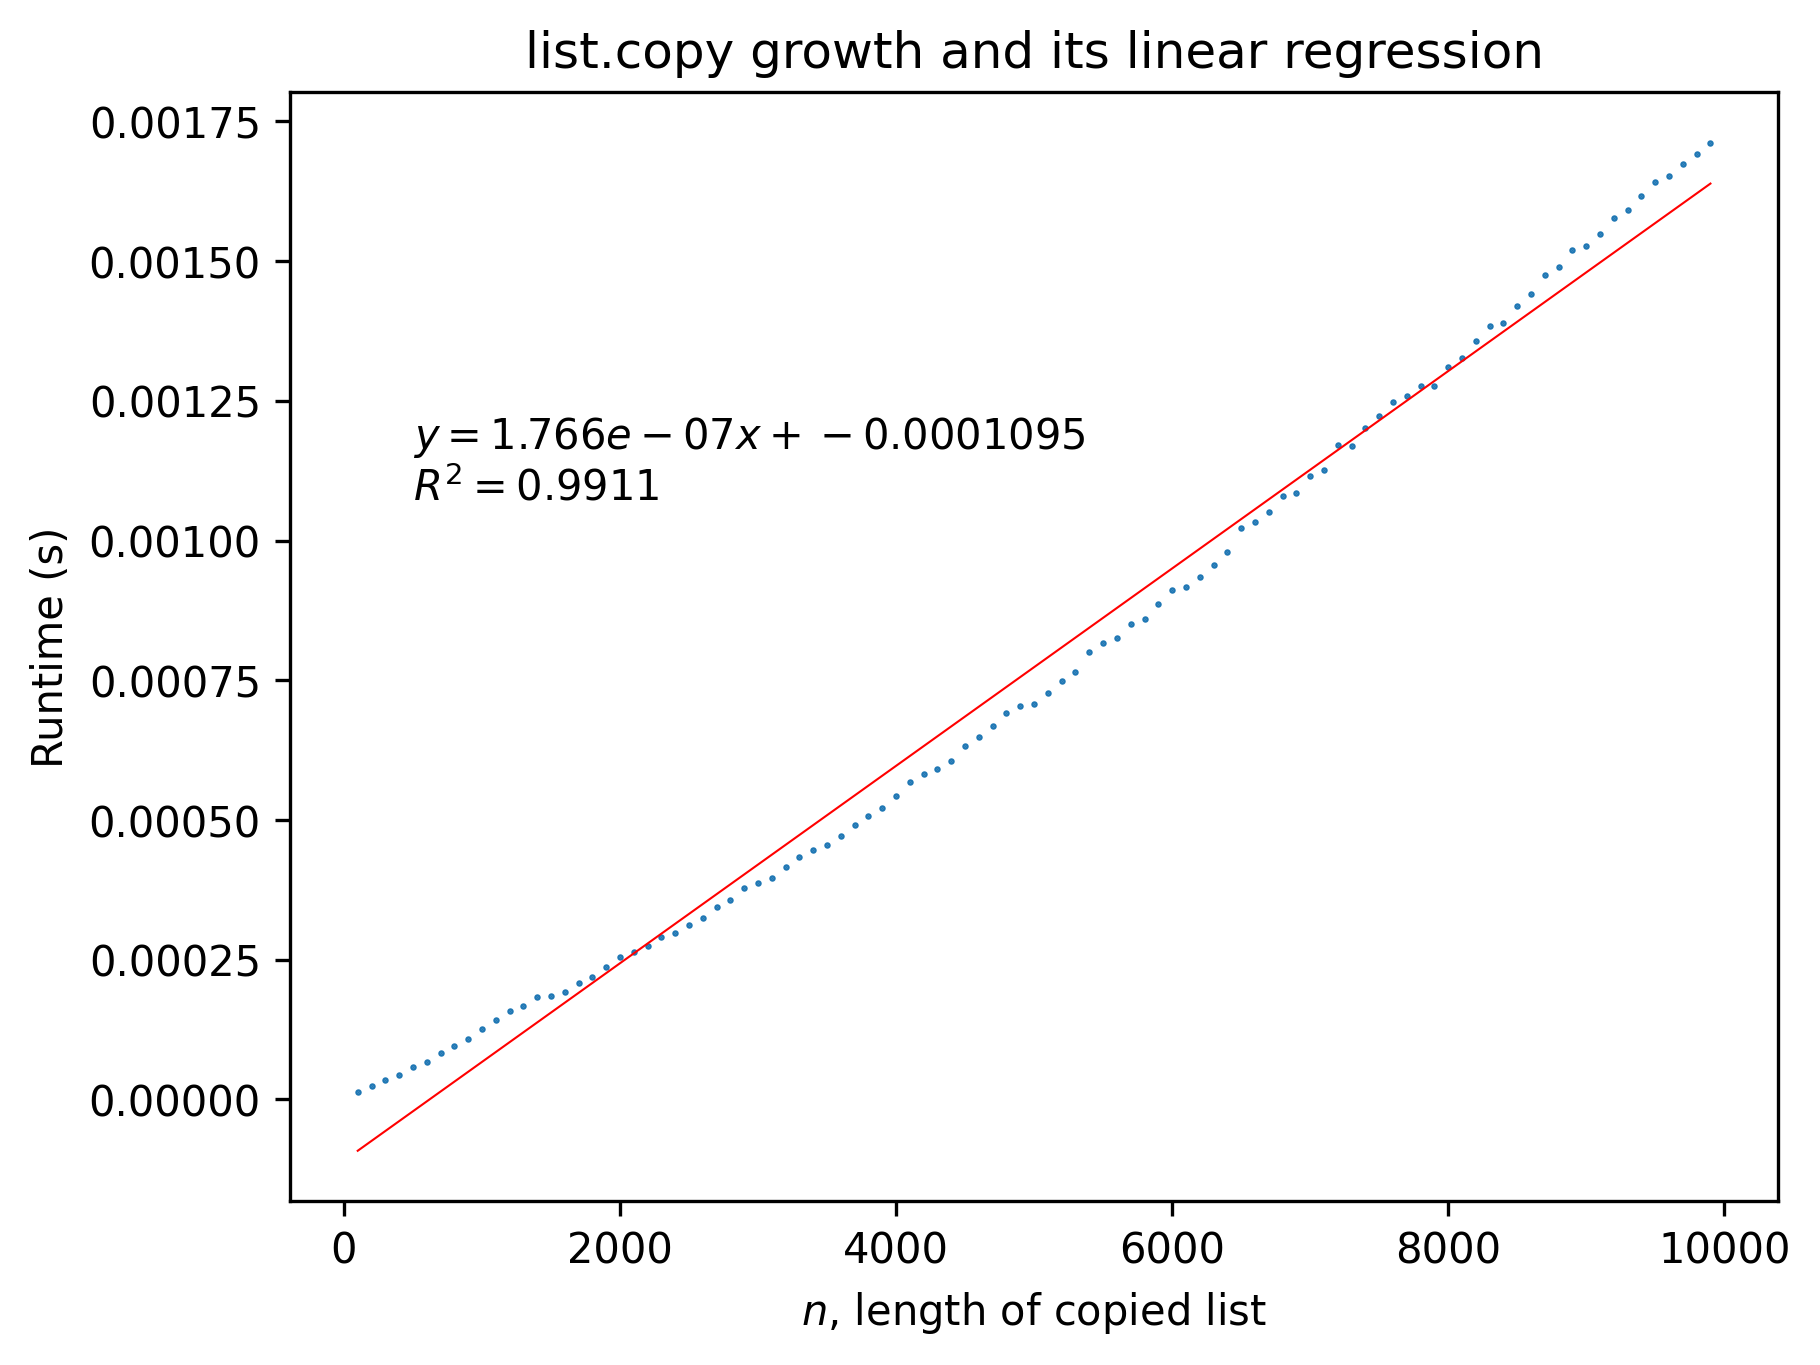
\includegraphics[width=0.8\linewidth]{copy-linreg.png}
  \centering
  \caption{\texttt{list.copy} runtime}
  \label{fig:copy-linreg}
\end{figure}

\subsubsection{Explanation}

\texttt{list.copy} copies the elements in a list one by one to a new location in
the memory. The only factor that affects the runtime is \( n \), the length of
the list, or, the amount of data. The more data needed to be copied, naturally
the longer the time \texttt{list.copy} needs.

\subsection{lookup}

\subsubsection{Prediction}

By the typical definition of arrays in common programming languages, random
array access is expected to have constant time complexity. Since the
builtin/native representation of array in Python is \texttt{list}, we expect
lookups by value for \texttt{list} in Python to also have constant time
complexity.

\subsubsection{Potential Problem}

Due to the expected huge amount of data generated during the experiment, it's
impossible to copy and paste the data into other tools like Excel and generate
the plot\footnote{Later in the experiment we did try and fail to do this}.
Therefore, we used a community Python library, \texttt{matplotlib} to plot the
graphs we needed. The timing data generated by our experiment is directly fed
and processed to the library within our Python module.

In addition, we believed that there will be a small portion of the data that
deffer from the majority. These outliers are caused by other programs running in
the background, different resource allocations by the operating system and so
on.

\subsubsection{Result}

The plotted graph matches our prediction. As shown in Figure \ref{fig:lookup},
the runtime of each list access is independent of which element is accessed.
\begin{figure}[H]
  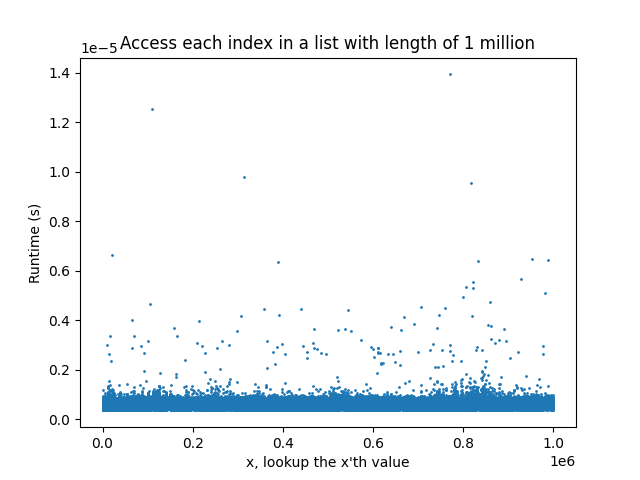
\includegraphics[width=0.8\linewidth]{lookup.png}
  \centering
  \caption{\texttt{list} access runtime}
  \label{fig:lookup}
\end{figure}

\subsection{\texttt{list.append}}

\subsubsection{Prediction}

The append method takes a constant amount of time to append each value to the
list, the running time stays the same throughout the one million
\texttt{list.append} calls. Similar to the lookups method, the
\texttt{list.append} method appends each element to the tail of the list, it
does not need to access any of the list or perform any operation. Therefore, we
predict the trend of the plotted dots to be constant, which would be reflected
as a horizontal line in the graph.

\subsubsection{Potential Problem}

As the same as the lookups, we will be dealing with a million data point at a
time. Transferring data in and out excel and the huge workload on the computer
would be our potential problems. Based on the method we summarized on the
previous test, we modified the code to fit our needs to get the plotted dot
graph for the Append method. Also, we believed that there must be a small
portion of the data that acts differently from the majority. Because there are
always other programs running in the background, it may affect the performance
of our operating system. As long as the incompatible data is relatively less
than the majority, the result is still reliable.

\subsubsection{Result}

The result graph is as neat as our prediction. Figure \ref{fig:append} overall
shows a straight horizontal line along with a few out of line data points. It
proves our guesses that the \texttt{list.append} method has a constant growth
order.
\begin{figure}[H]
  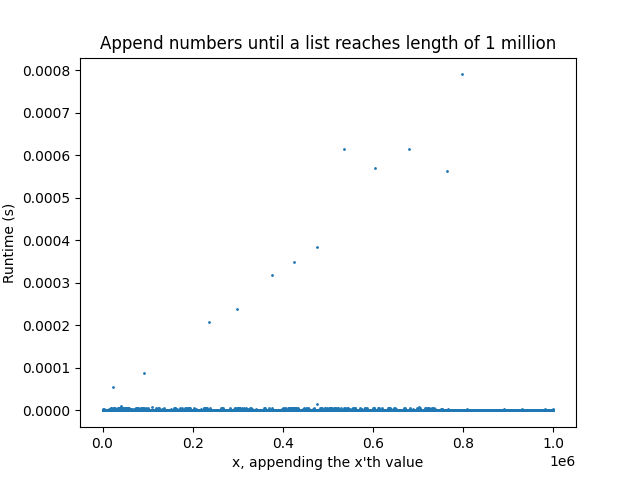
\includegraphics[width=0.8\linewidth]{append.png}
  \centering
  \caption{\texttt{list.append} runtime}
  \label{fig:append}
\end{figure}

\subsubsection{Extra Experiment plan}

In the previous experiment for \texttt{list.append}, we used the method to
append one million integers in an increasing order into a \texttt{list}. To
further investigate the behaviours and runtime of \texttt{list.append}, we
decided to instead append a fixed string into a \texttt{list} 1 million times.
We predicted the outcome to be the same as that of the previous experiment,
because the runtime of an algorithm is usually independent of the data type
on which the algorithm is used.

\subsubsection{Extra Experiment Result}

After appending one million strings to the list and generating the scatter plot
of the running time, we proved our guess that the runtime of append does not
depend on the data type, as shown in Figure \ref{fig:append-string}. To
conclude, the appended data consumes the same time, no matter what the data type
is. The running time of append grows in \( \mathcal{O}(1) \).
\begin{figure}[H]
  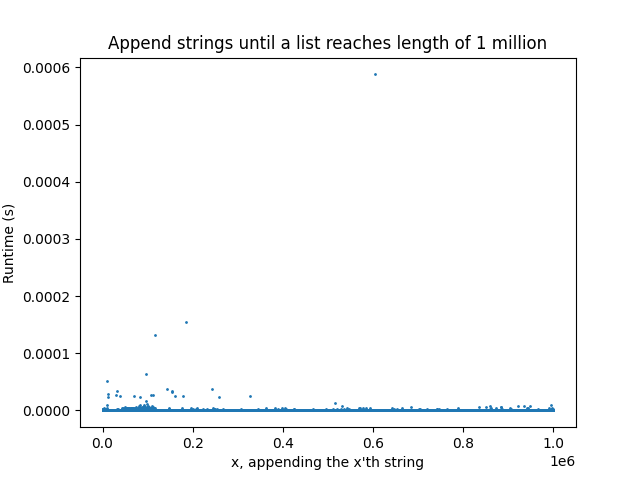
\includegraphics[width=0.8\linewidth]{append-string.png}
  \centering
  \caption{\texttt{list.append} runtime, operated on strings}
  \label{fig:append-string}
\end{figure}

\subsubsection{Comparison to Official Runtime Claims}

All of our experiment results are consistent with the Python complexity claims,
namely, \texttt{list.copy} has a complexity of \( \mathcal{O}(n) \), lookups
(index) has a complexity of \( \mathcal{O}(1) \), and \texttt{list.append} has a
complexity of \( \mathcal{O}(1) \).

\end{document}